

\chapter{Corda Vibrante}

\section{Introduzione}

Obiettivo di questo esperimento è lo studio della propagazione di onde elastiche su una corda \textbf{fissata agli estremi}, sotto l'azione di una forzante con andamento sinusoidale. \textbf{Verifichiamo} la dipendenza della frequenza dell'onda ($\nu_n$) \textbf{dalla lunghezza della corda, dalla sua massa lineare ($\mu$)} e dalla tensione ($T$) applicata su di essa.
\textbf{Tali grandezze sono infatti legate dalle seguenti relazioni:}
\begin{center}
\begin{tabular}{c c c}
$
v= \sqrt{\frac{T}{\mu}} 
$
&
$
v= \nu_{n} \lambda_n
$ 
&
$
\lambda_n= \frac{2L}{n} 
$
\\
\end{tabular}
\end{center}

da cui:

\begin{equation}
\nu_n=\frac{n}{2L}\sqrt{\frac{T}{\mu}}
\end{equation}


\section{Strumenti}

\section{Ricerca delle armoniche}

Nella prima parte dell'esperienza, dopo aver trovato la frequenza di risonanza, abbiamo misurato le frequenze relative alle prime cinque armoniche di una corda vibrante di lunghezza $=111 cm$ e peso $5.21 g$ posta sotto una tensione $T$. La lunghezza $l$ è la distanza tra i punti di sospensione della corda: il primo coincidente nel punto di applicazione della forzante, il secondo è il punto di tangenza della carrucola.  
\\

Abbiamo ripetuto la misurazione sottoponendo la corda a quattro differenti forze di tensione (ottenute appendendo un peso ad una delle estremità della corda, come illustrato in figura) e per due corde di masse lineari $\mu$ differenti. 
\\
Nel seguente grafico, mostriamo la relazione tra la frequenza $\nu$ e il numero di armonica $N$. La relazione è lineare ed è la seguente equazione:
$$ \nu_n = 16.1n + 0.31 $$ 
\\
con $A= 0.31$, $\sigma_A=  0.93$ e $B=16.1, \sigma_B = 0.28 $ ricavati con il metodo dei minimi quadrati. 

\begin{center}

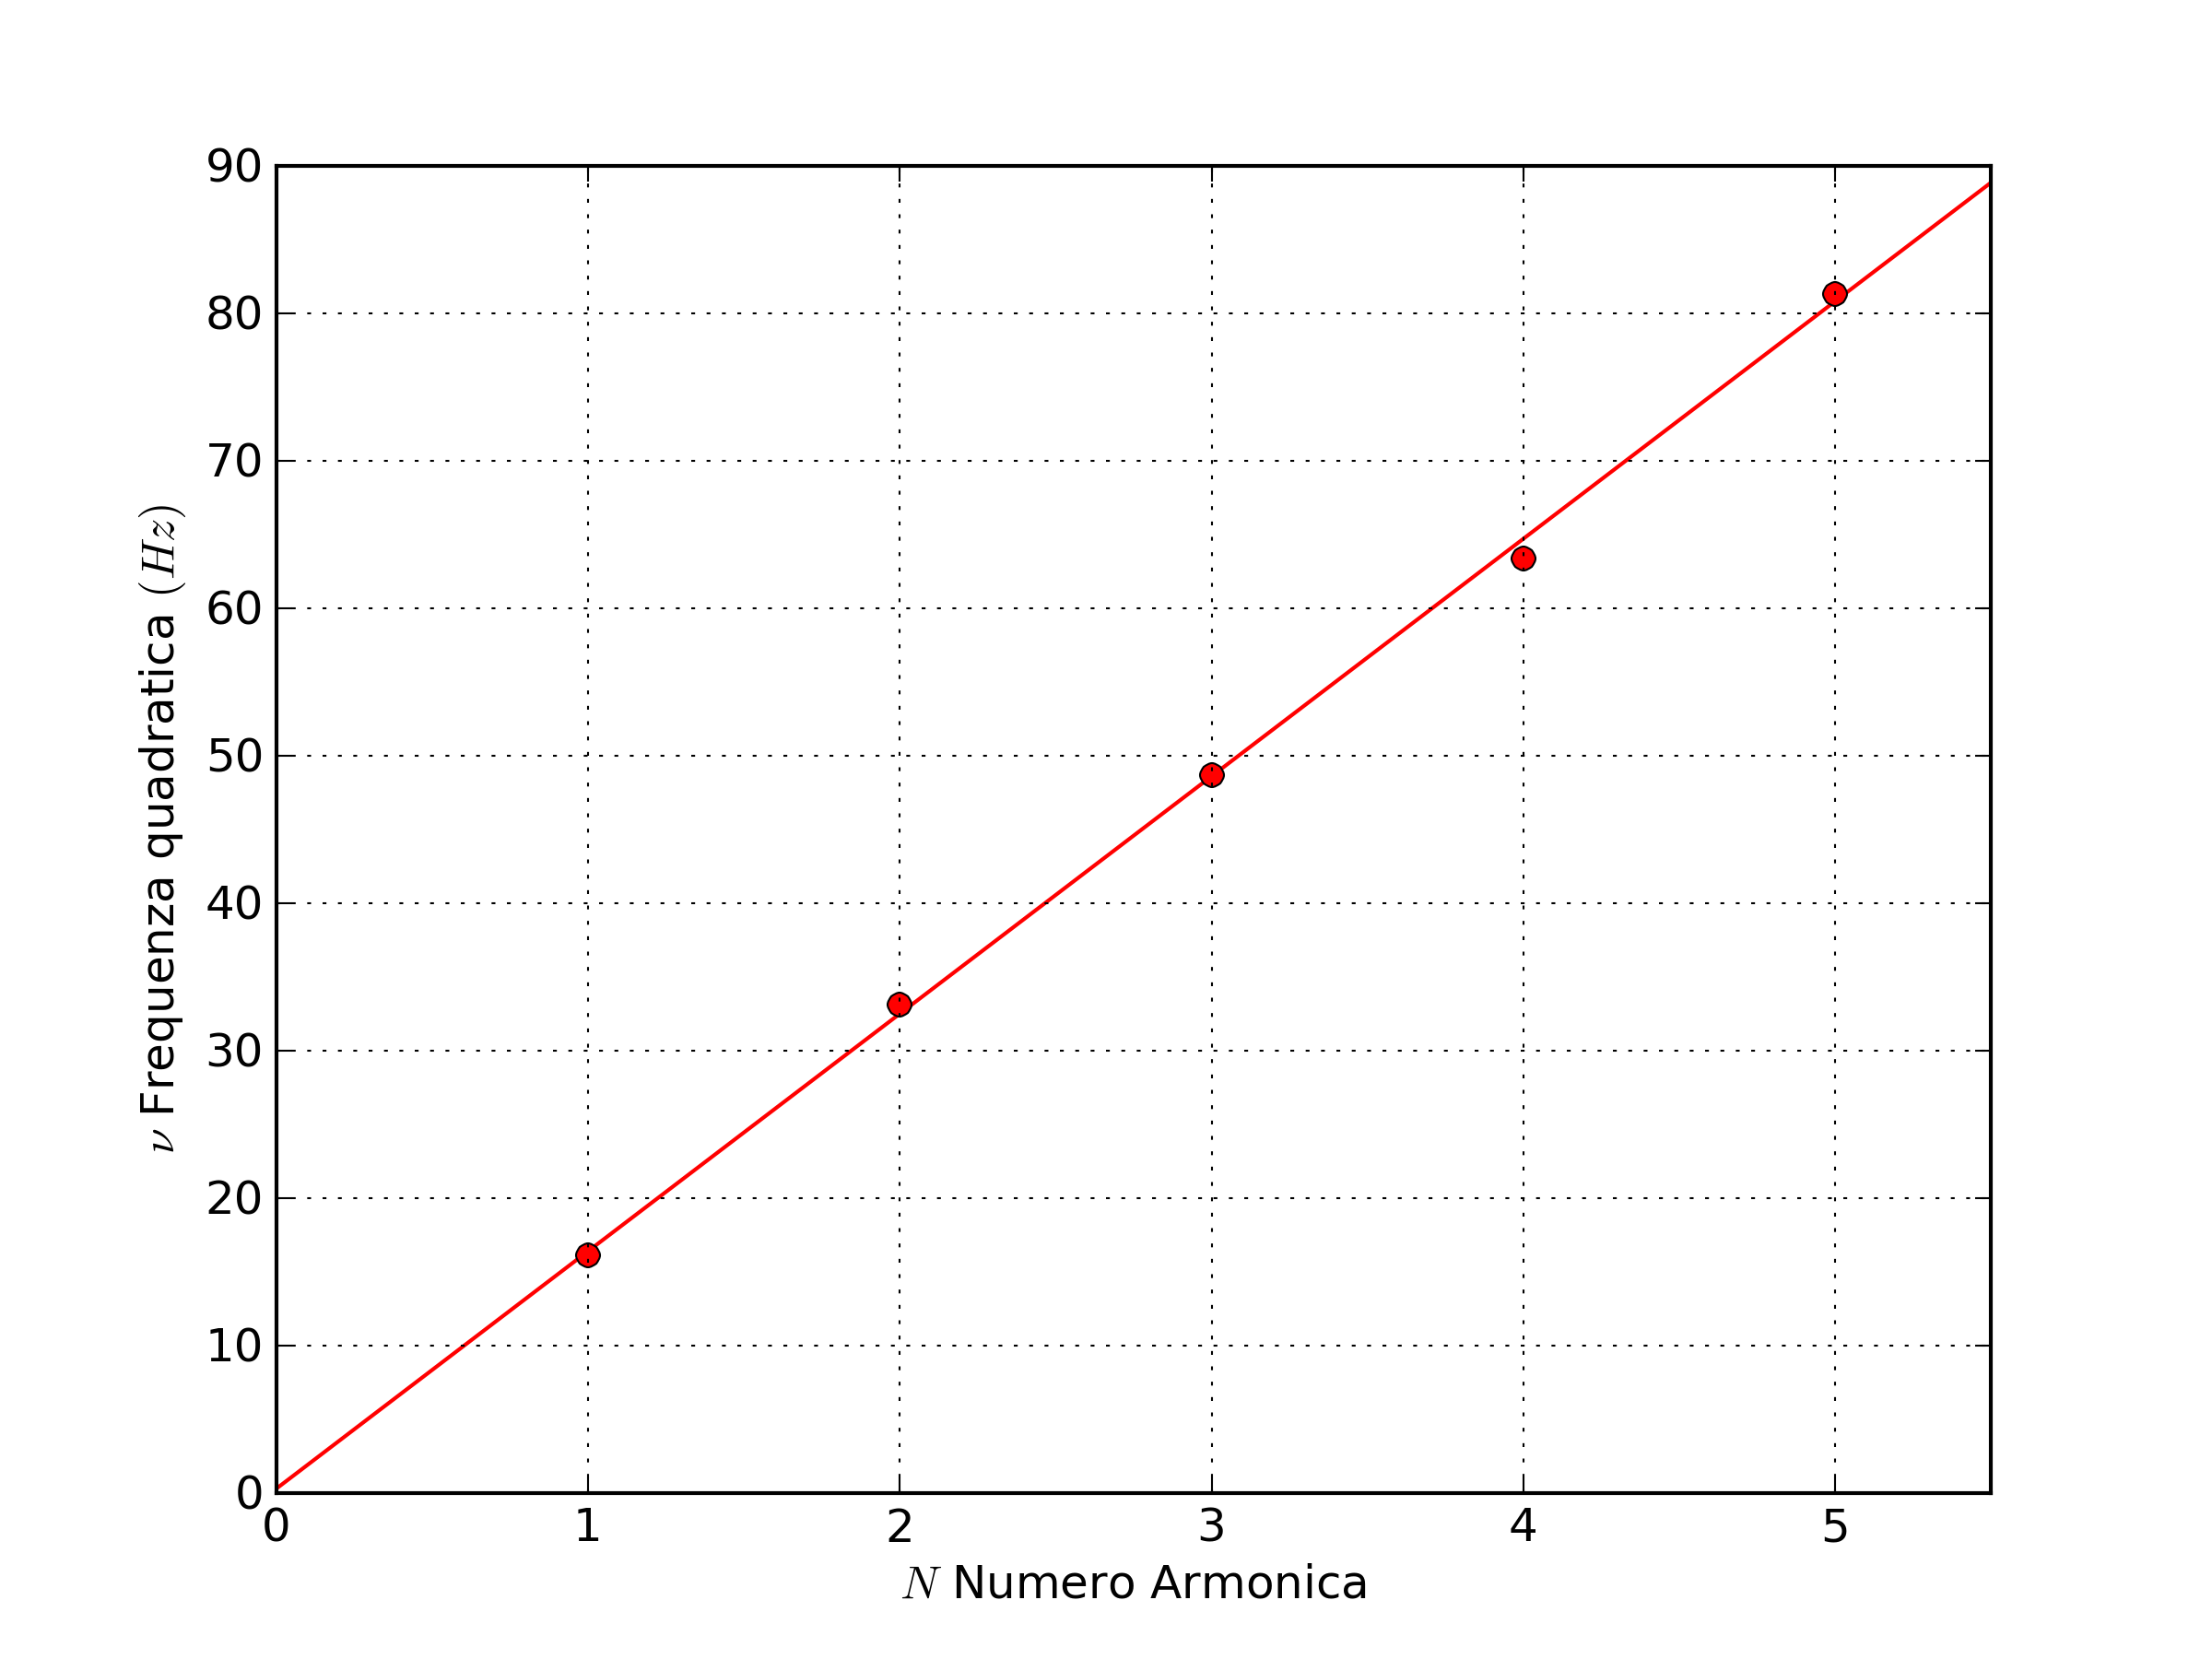
\includegraphics[scale=0.5]{../grafici/corda_1armonica}
\end{center}
Questo grafico è stato ricavato dalla corda A sottoposta ad una tensione $\tau=g\cdot250g$. Di seguito tutti i valori della frequenza di risonanza in funzione del numero di armonica e della tensione $\tau$ per valori crescenti della massa.

\begin{center}
\begin{tabular}{c   |  c}
\textbf{Corda A }
\begin{tabular}{ c | c | c | c | c | c }
Massa($g$) & 1 & 2 & 3 & 4 & 5\\
\midrule
550 & 23.7 & 45.5 & 71.3 & 94.6 & 119.6\\
450 & 21,4 & 42,6 & 63,4 & 85,3 & 108,9\\
350 & 19.6 & 37.8 & 57.4 & 76.3 & 95.0\\
250 & 16.1 & 33.1 & 48.7 & 63.4 & 81.3 \\
\end{tabular}
&
\textbf{Corda B}
\begin{tabular}{ c | c | c | c | c | c }
Massa($g$) & 1 & 2 & 3 & 4 & 5\\
\midrule
1050 & 19.3 & 38.4 & 56.1 & 75.2 & 94.7 \\
550 & 14.1 & 26.8 & 40.8 & 55.0 & 69.9 \\
450 & 13.1 & 25.4 & 38.9 & 51.7 & 64.2\\
350 & 10.9 & 22.8 & 35.2 & 46.9 & 58.3\\
\end{tabular}

\end{tabular}
\end{center}
\section{Dipendenza dalla tensione}
Dall'equazione $1.1$ si deduce la dipendenza quadratica tra la tensione $\tau$ e la frequenza $\nu$. 
Verifichiamo questa dipendenza utilizzando i dati della seconda armonica misurati precedentemente. 
\begin{center}
\begin{tabular}{c | c}

\textbf{Corda A}
\begin{tabular}{c|c}
Tensione $N$ & Frequenza $Hz$ \\
\midrule
2.45 & 33.1\\
3.43 & 37.8\\
4.41 &42.6\\
5.39 &45.6\\
\end{tabular}
&\textbf{
Corda B}
\begin{tabular}{c|c}
Tensione $N$ & Frequenza $Hz$ \\
\midrule
3.45 & 22.8\\
4.41 & 25.4\\
5.39 & 26.8\\
10.3 & 38.4\\
\end{tabular}
\\
\end{tabular}
\end{center}

Essendo il numero dei dati troppo ridotto per essere interpolato con successo dalla curva corrispondente ($1.1$), consideriamo un'interpolazione lineare di tipo $y = mx$ dove   $y= \nu^2$ e $x = \tau$.
\\
Utilizziamo il metodo dei minimi quadrati, ottenendo per la\textbf{ corda A} $m_A = 403.95$ con incertezza $\sigma_m =0.03$ e per la \textbf{corda B} $m_B=143.0$ con incertezza $\sigma_m$.  Di seguito il grafico che rappresenta la relazione tra $\nu^2$ e $\tau$.

\begin{center}
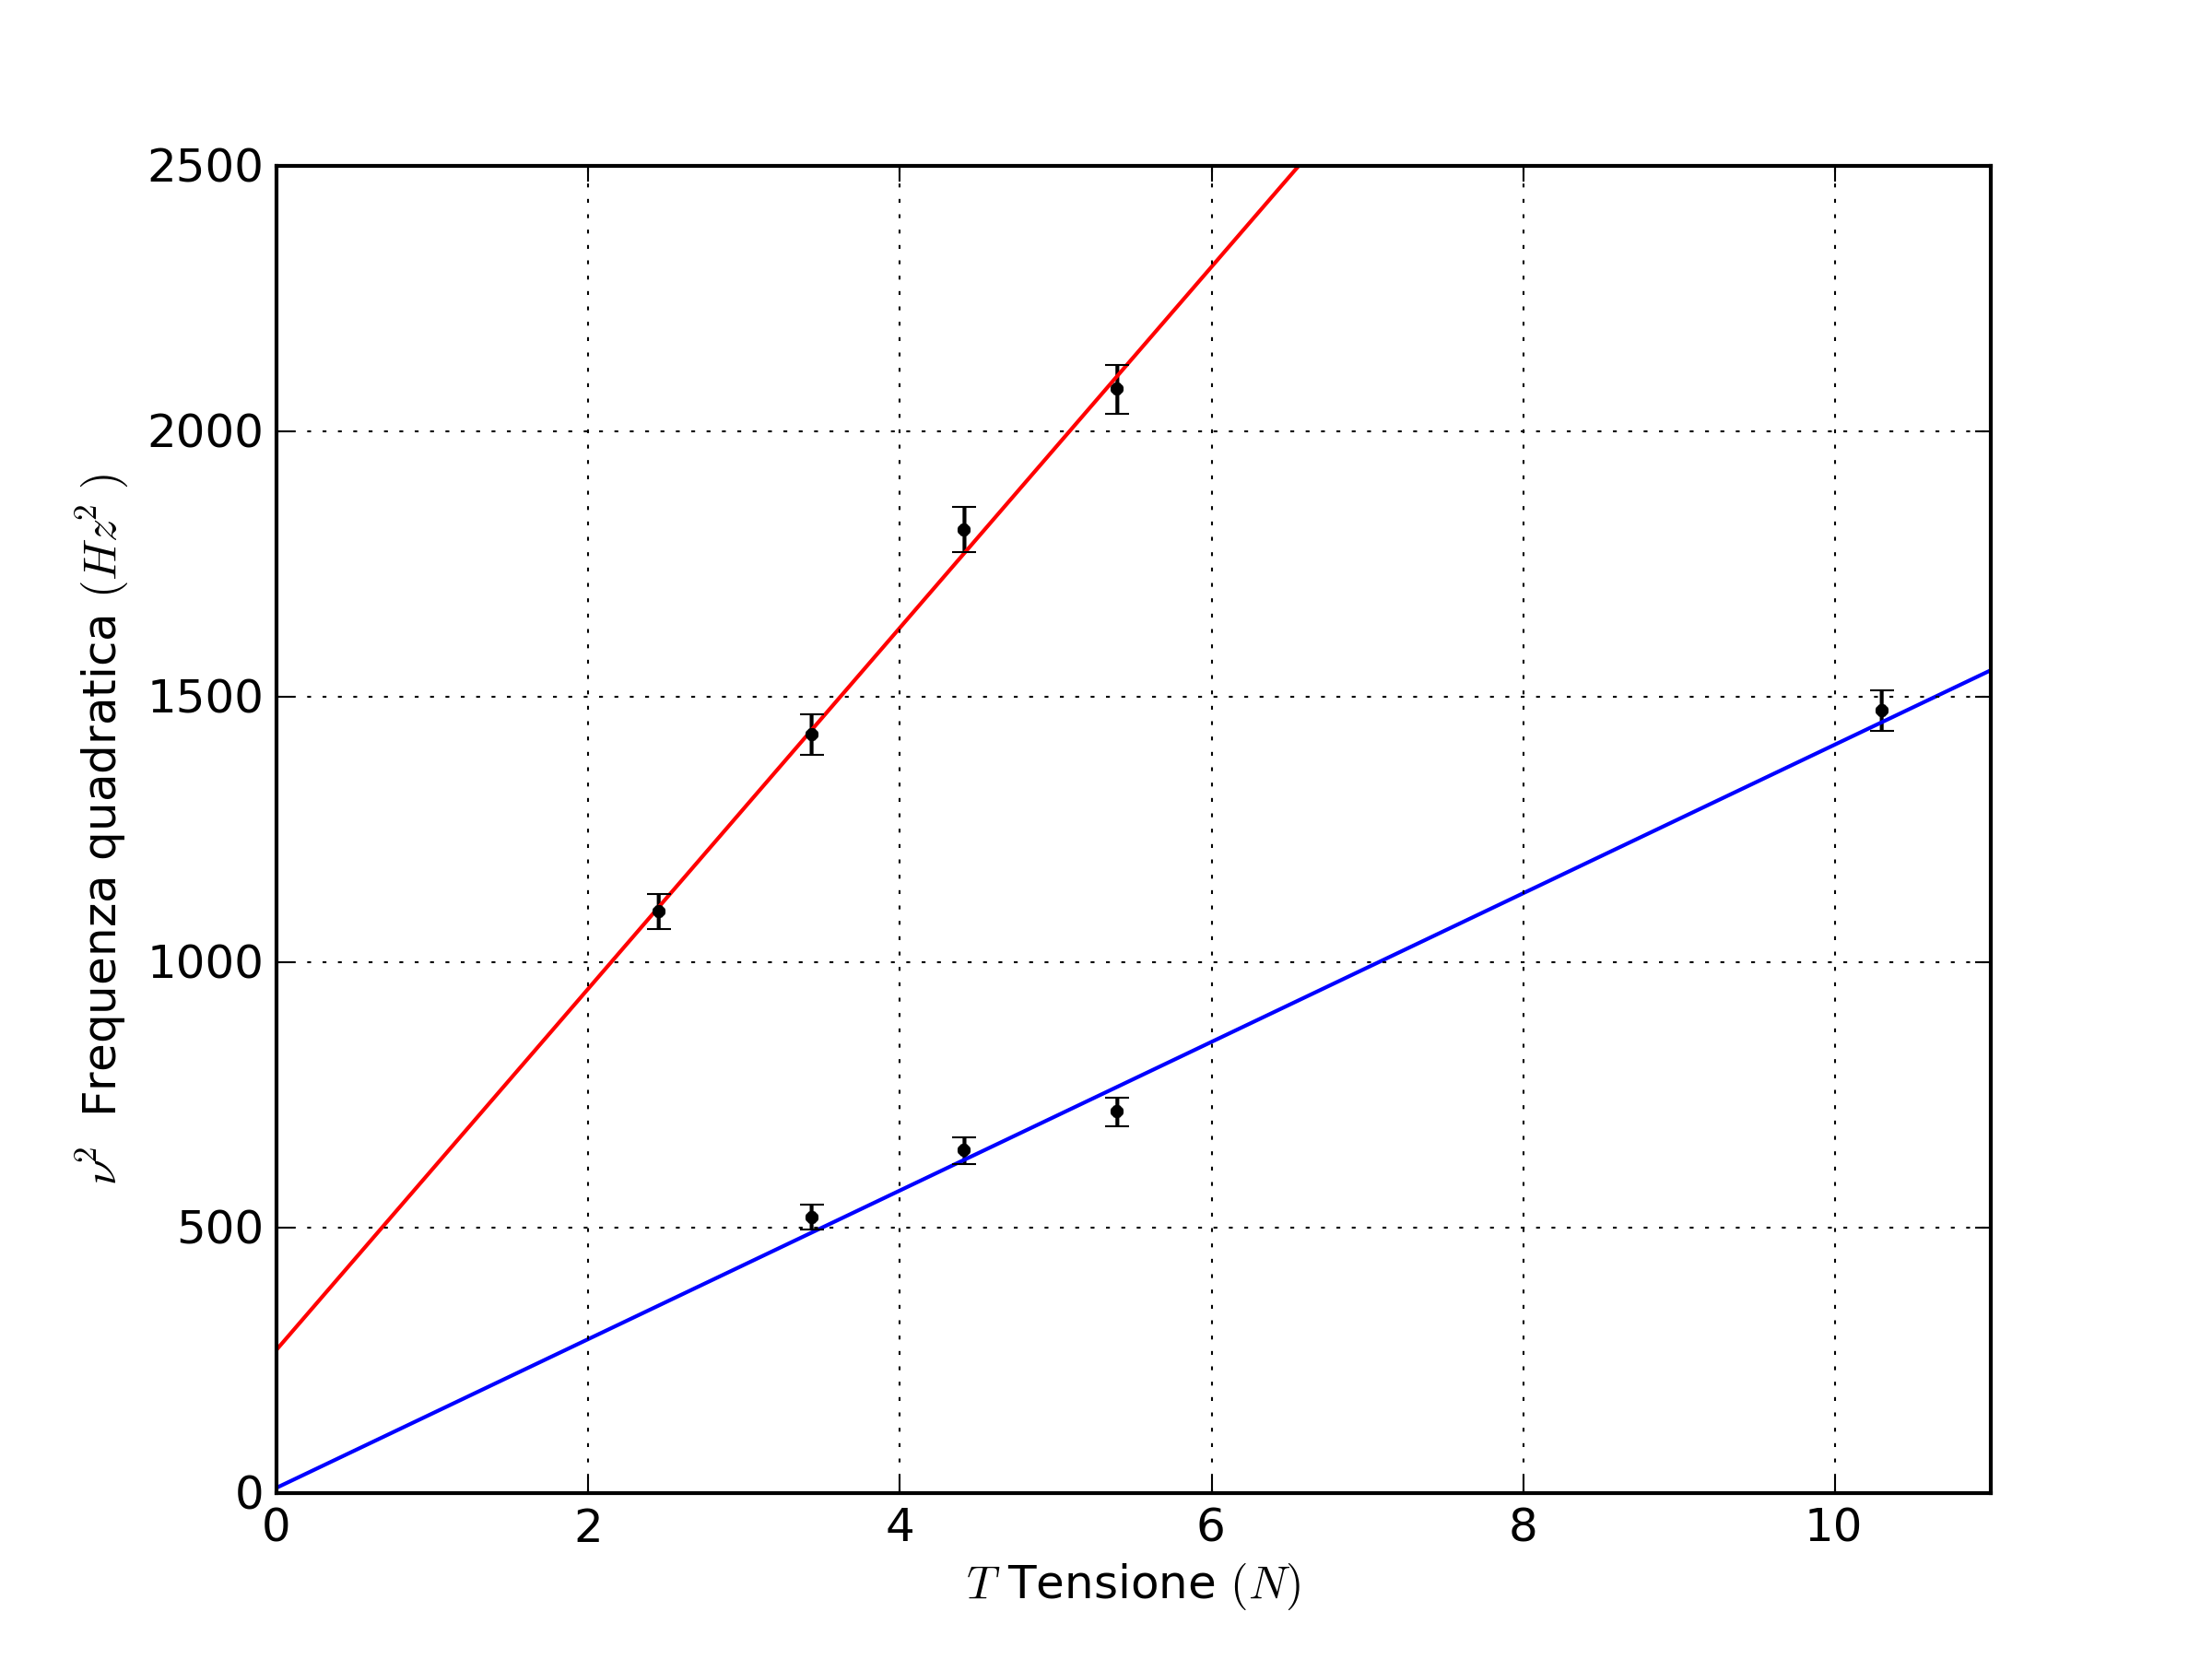
\includegraphics[scale=0.5]{../grafici/corda_tensione}
\end{center}



\section{Dipendenza dalla lunghezza}
Sempre dall'equazione $1.1$, si deduce la proporzionalità inversa tra la frequenza $\nu$ e la lunghezza $l$. 
Corda A,550g

\begin{center}


\begin{tabular}{c|c}
L($cm$) & $\nu (Hz) $ \\
\midrule
105 & 24.6\\
111 & 23.7\\
116.5 & 22.8 \\
122.5 & 20.9 \\
131.5 & 20.1 \\
\end{tabular}
\end{center}

In tabella sono riportati i dati della frequenza delle prima armonica, 
Corda B,1050g

\begin{center}
\begin{tabular}{|c|c|}
\toprule
Lunghezza (m) & Frequenza (Hz) \\
\midrule
1.10 & 19.33 \\
1.15 & 18.25 \\
1.17 & 17.75 \\
1.22 & 17.00 \\
1.34 & 15.69 \\
1.53 & 13.92 \\
1.60 & 12.96 \\
0.91 & 22.83 \\
0.75 & 27.85 \\
0.60 & 35.00 \\
0.50 & 42.67 \\
\bottomrule
\end{tabular}
\end{center}

Inserendo questi dati su di un grafico, e interpolando la curva con Sage, troviamo il seguente grafico.

\includegraphics[scale=0.75]{"../grafici/CordaPrimaArmonica"}

Nota: $\rho$ è lasciato parametro libero, mentre invece $\tau$ è pari a 10.3 N, dato da un peso di 1.050 Kg sospeso a un'estremità della corda.
